%-- Intro --%

\begin{tframe}{Introduction}

\vspace{0.5cm}
Digital images are easy to manipulate thanks to the availability of the \textbf{powerful editing software} and \textbf{sophisticated digital cameras}.

\vspace{1cm}

\begin{minipage}{\textwidth}
\begin{columns}[T]
\begin{column}{0.5\textwidth}
\vspace{0.1cm}
The development of methods for verifying \textbf{image authenticity} is a real need in forensics.

\vspace{0.8cm}
\textbf{Purpose}: to detect image splicing  aimed at \emph{deceiving} the viewer.
\end{column}
\begin{column}{0.4\textwidth}

\includegraphics[width=0.8\textwidth]{images/image-editing.jpg}
\end{column}
\end{columns}
\end{minipage}

\end{tframe}

%-- Image compositions --%

\begin{tframe}{Forgery detection}
\vspace{0.2cm}
Image splicing detection techniques are based on \textit{inconsistencies}:
\vspace{0.3cm}
\begin{enumerate}
\item \textbf{Image resampling, copy-paste}: deduced from image metadata.
\vspace{0.3cm}

\item \textbf{Compression-based inconsistencies}: JPEG compression introduces blocking artifacts. Manufacturers of digital cameras and image processing software typically use different JPEG quantization tables.
\vspace{0.3cm}

\item  \textbf{Neighboring pixels relationship inconsistencies}: when an image is spliced some artifacts can be created.
\vspace{0.3cm}
\item \textbf{Intrinsic image properties inconsistencies}: e.g. scene lights, shadows or perspective.
\end{enumerate}

\end{tframe}

%-- Light based detection --%

\begin{tframe}{Lighting-based inconsistencies}
\vspace{0.2cm}
Methods based on \textbf{lighting inconsistencies} are particularly \emph{robust}: a perfect illumination adjustment in a image composition is very hard to achieve.
\vspace{0.3cm}
\begin{center}
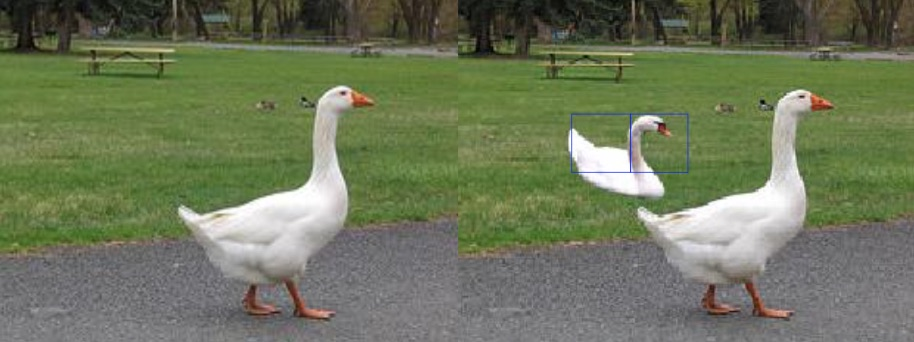
\includegraphics[width=0.5\textwidth]{images/ducks.jpg}
\vspace{0.1cm}
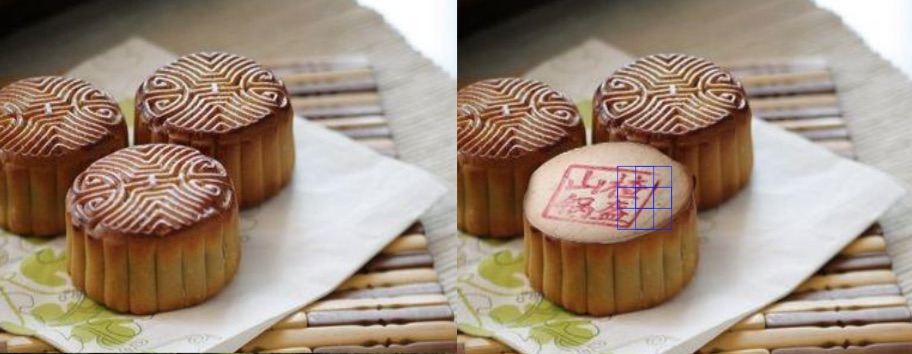
\includegraphics[width=0.5\textwidth]{images/cakes.jpg}
\end{center}
\end{tframe}

\begin{tframe}{Lighting-based inconsistencies}
\vspace{0.1cm}
These methods can be divided into two types of approaches:
\vspace{0.2cm}
\begin{enumerate}
\item \textbf{Object light source inconsistencies}: detected using \emph{shadows}, \emph{face geometry}, \emph{generic object surfaces}.
\vspace{0.2cm}

\item \textbf{Illuminant colors inconsistencies}: {\small assuming that a scene is lit by the same light source, all objects must have the same illuminant colors.}
\vspace{0.2cm}
\begin{enumerate}
\item \textit{Specular dichromatic reflectance models}
\vspace{0.1cm}
\item \textit{Illuminant Maps (IMs)}
\end{enumerate}
\end{enumerate}
\begin{center}
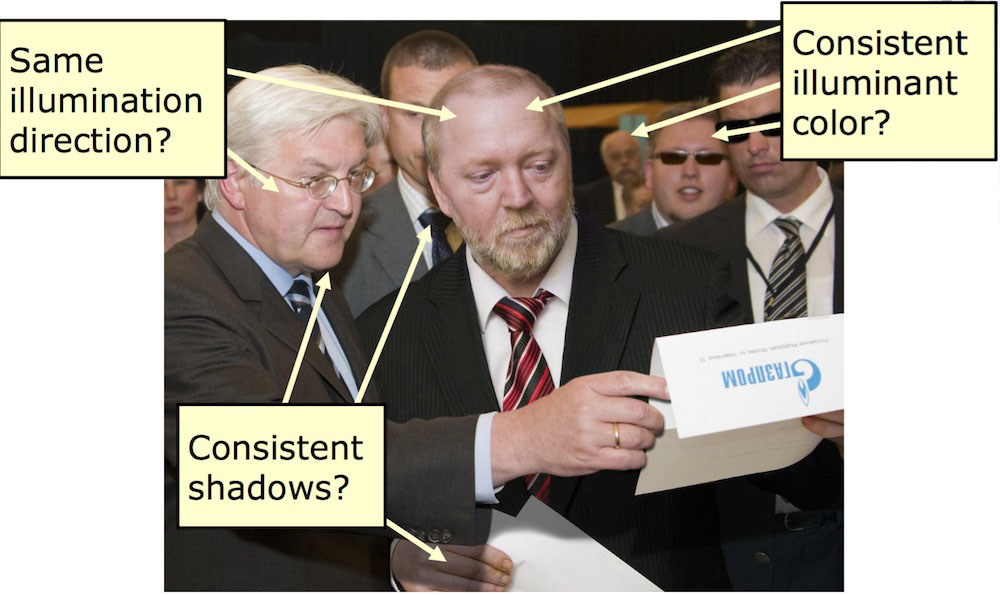
\includegraphics[width=0.4\textwidth]{images/lighting-based.jpg}
\end{center}
\end{tframe}


\begin{tframe}{Illuminant Maps estimation}
\vspace{0.2cm}
For the Illuminant Maps estimation, two different techniques are used: 
\vspace{0.3cm}
\begin{enumerate}
\item A \emph{statistical-based} approach using \textbf{Generalized Grayworld Estimate (GGE)} algorithm.
\vspace{0.2cm}
\item A \emph{physics-based} approach using \textbf{Inverse-Intensity Chromaticity (IIC)} method.
\end{enumerate}

\begin{center}
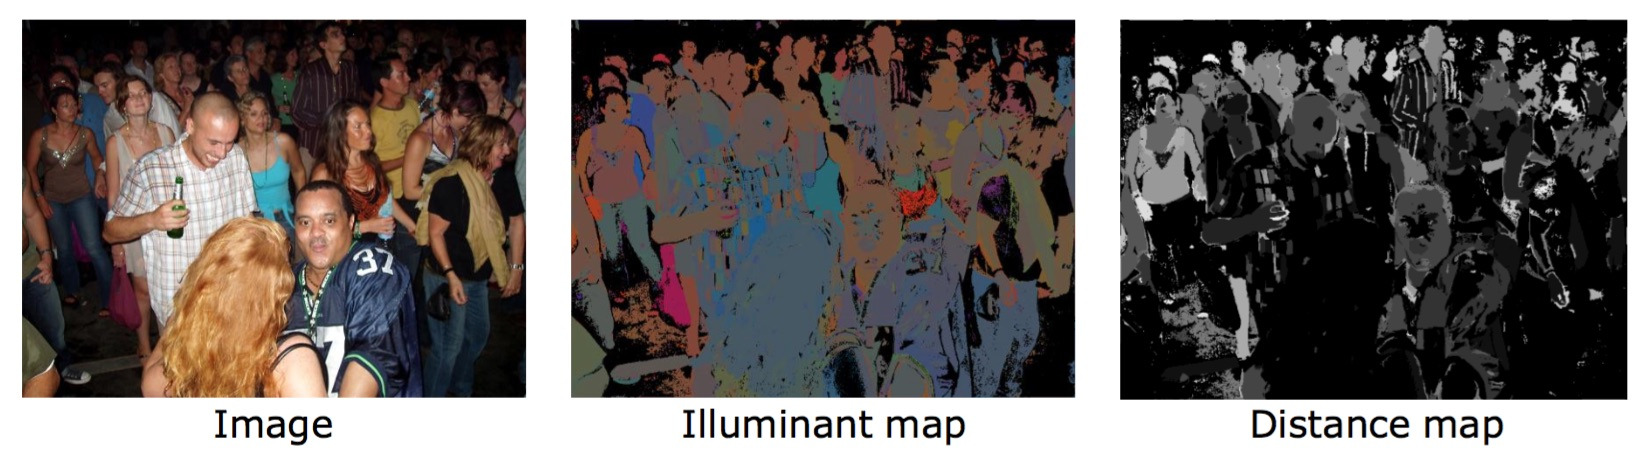
\includegraphics[width=0.7\textwidth]{images/riess.jpg}
\end{center}
\end{tframe}


\begin{tframe}{Generalized Greyworld Estimate (GGE)}
\textbf{Generalized Greyworld Estimate} is proposed in [2] as a combination of the \emph{Grey-World} and \emph{Grey-Edge method}s aimed to evaluate \textbf{color constancy}.

\vspace{0.3cm}
The main premise behind it is that in a normal well color balanced photo, the \textbf{average} of all the colors is a neutral gray. Therefore, it assumes that the \emph{Minkowski norm} of the derivative of the reflectance in a scene is \textbf{achromatic}.

\begin{equation}
k\textbf{e}^{n, p, \sigma} = (\int |\frac{\vartheta^{n}\textbf{f}^{\sigma}(\textbf{x})}{\vartheta\textbf{x}^{n}}|^{p}  d\textbf{x})^{\frac{1}{p}}
\end{equation}
\begin{footnotesize}
where $\textbf{x}$ denotes a pixel coordinate, $k$ is a scale factor, $|\cdot|$ is the absolute value operator, $\vartheta$ the partial differential operator, $\textbf{f}^{\sigma}$ is the observed intensities at position $\textbf{x}$, smoothed by a Gaussian kernel $\sigma$, $p$ is the \emph{Minkowski norm}, and $n$ is the derivative order.
\end{footnotesize}
\end{tframe}

\begin{tframe}{Generalized Greyworld Estimate (GGE)}

The illuminant estimation of (1) is a framework for low-level based illuminant estimation based on three variables:
\begin{enumerate}
\item The order $n$ of the image structure.
\item The Minkowski norm $p$ which determines the relative weights of the multiple measurements from which the final illuminant color is estimated.
\item The scale of the local measurements as denoted by $\sigma$.
\end{enumerate}
\vspace{0.2cm}
\textbf{Advantages}:
\begin{itemize}
\item the Minkowski norm of RGB values or derivatives can be computed\emph{ extremely fast}
\item the method does not require an image database taken under a \textbf{known light source}
\end{itemize}

\end{tframe}


\begin{tframe}{Inverse-Intensity Chromaticity (IIC)}
Extension of the \textbf{dichromatic reflectance model}, which states that \emph{the amount of light reflected from a point, $\textbf{x}$, of a dielectric, non-uniform material is a linear combination of diffuse reflection and specular reflection}.

\vspace{0.2cm}

Given an image taken with a \textbf{RGB camera}, the response $I_c(\textbf{x})$ for each color filter $c \in \{R, G, B\}$ is

$$
I_c(\textbf{x}) = m_d(\textbf{x})B_c(\textbf{x}) + m_s(\textbf{x})G_c(\textbf{x})
$$

\begin{small}
where $m_d$ and $m_s$ are geometric parameters of \textbf{diffuse and specular reflection}.
\vspace{0.2cm}

Let $\Delta_c(\textbf{x})$ and $\Gamma_c(\textbf{x})$ be the diffuse and \textbf{specular chromaticity}: $\Delta_c(\textbf{x}) = \frac{B_c(\textbf{x})}{\sum_{i in \{R, G, B\}} B_i(\textbf{x})}$ and $\Gamma_c(\textbf{x}) = \frac{G_c(\textbf{x})}{\sum_{i in \{R, G, B\}} G_i(\textbf{x})}$
\end{small}

\end{tframe}

\begin{tframe}{Inverse-Intensity Chromaticity (IIC)}

In this model, the intensity $I_c(\textbf{x})$ and the chromaticity $\sigma_c(\textbf{x})$ of a color channel $c \in \{R, G, B\}$ at pixel position $\textbf{x}$ are related by

\begin{equation}
\sigma_c(\textbf{x}) = p_c(\textbf{x}) \frac{1}{\sum_{i \in \{R, G, B\}} I_i(\textbf{x})} + \Gamma_c(\textbf{x})
\end{equation}
\vspace{0.2cm}

\begin{small}
where $p_c(\textbf{x}) = w_d(\textbf{x}) \sum_i B_i(\textbf{x}) (\Delta_c(\textbf{x}) - \Gamma_c(\textbf{x}))$ 
\end{small}

\begin{center}
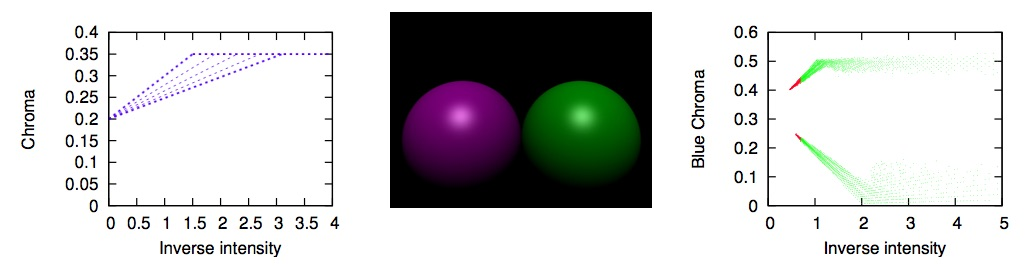
\includegraphics[width=0.6\textwidth]{images/iic.jpg}
\end{center}
The \emph{domain} of the line is determined by $\frac{1}{\sum_i I_i(\textbf{x})}$ and the \emph{range} is given by $0 \leq \sigma_c \leq 1$. Domain and range together form the \textbf{inverse-intensity chromaticity (IIC) space}.
\end{tframe}

\begin{tframe}{Proposed approach}

\begin{itemize}
\item \textbf{Face forgery detection module}: specifically for detecting forgeries involving people. Based on the work presented by Carvalho et al. [1].

\item \textbf{Regional forgery detection module}: image content independent. Based on the work presented by Fan et al. [2]
\end{itemize}

\end{tframe}

\begin{tframe}{Face forgery detection module}

\begin{center}
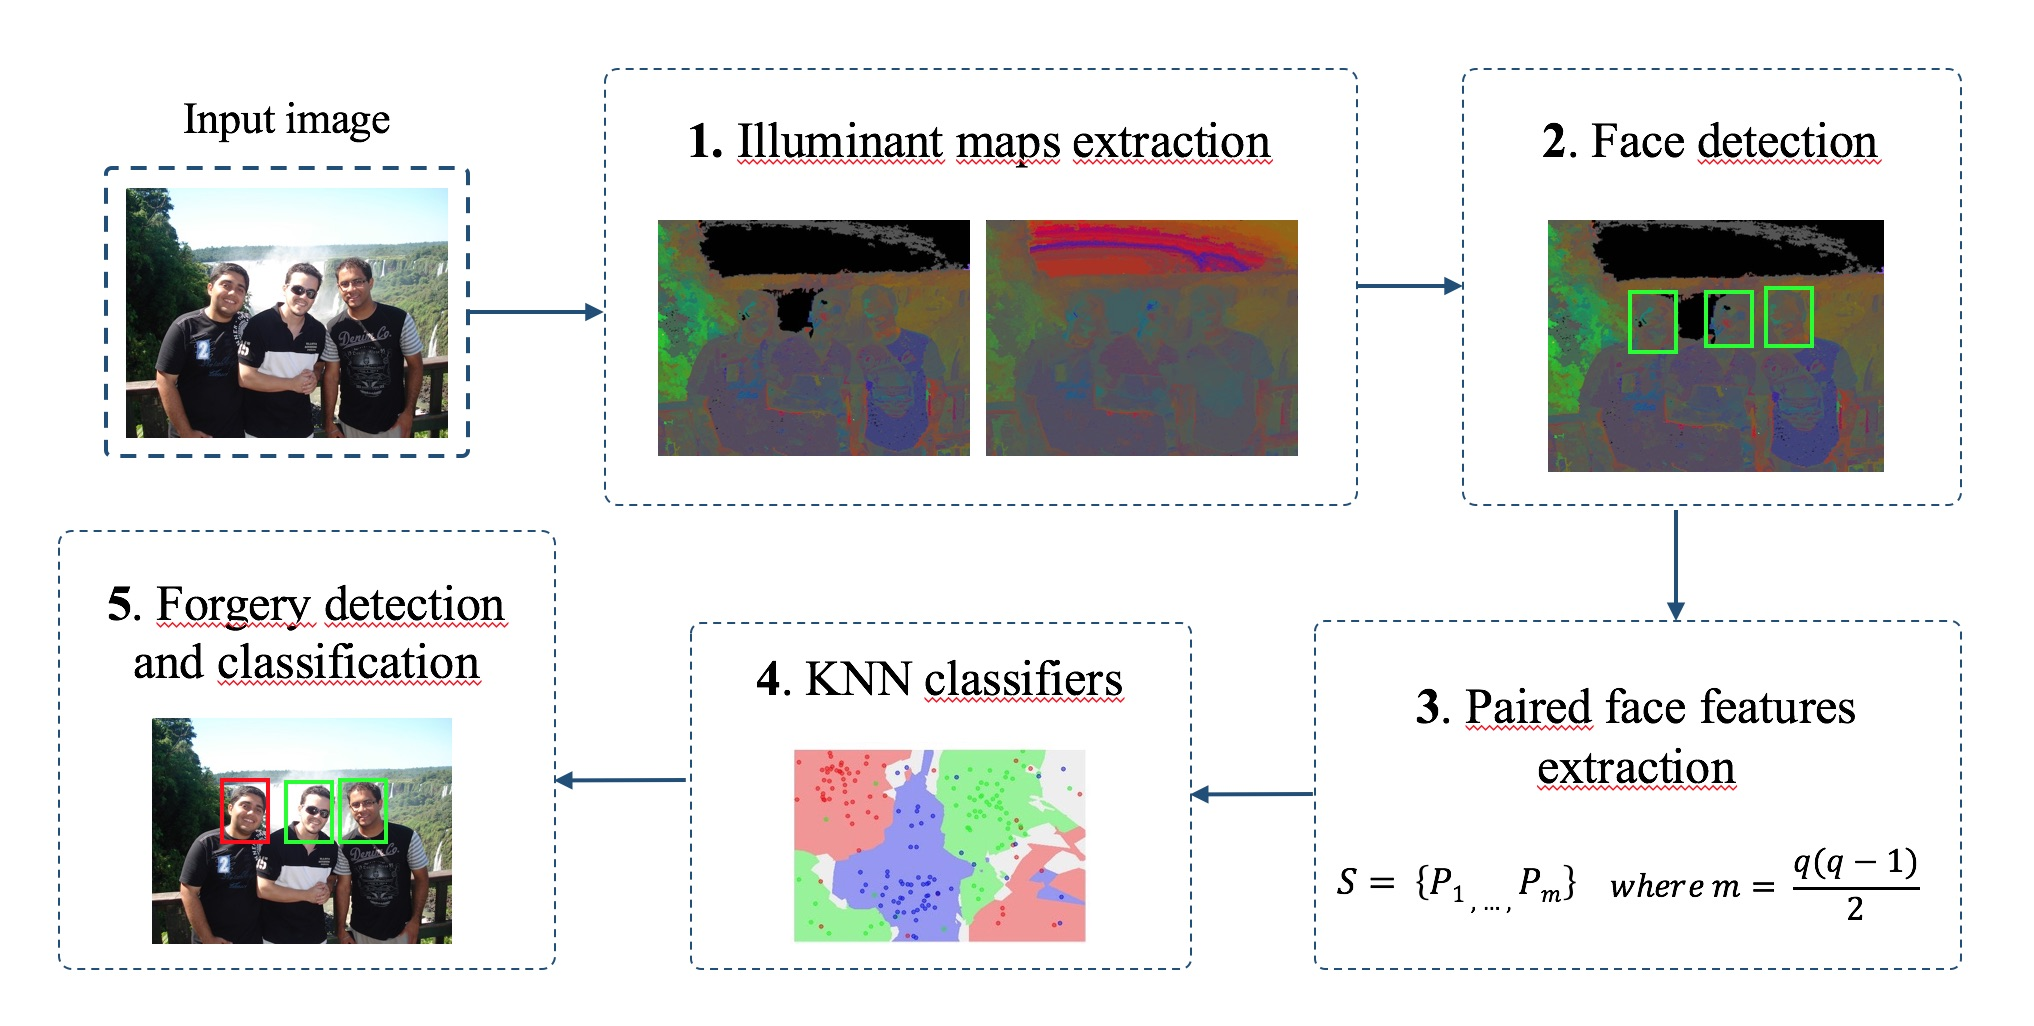
\includegraphics[width=1\textwidth]{images/pipeline_faces.jpg}
\end{center}
\end{tframe}


\begin{tframe}{Region forgery detection module}
\begin{center}
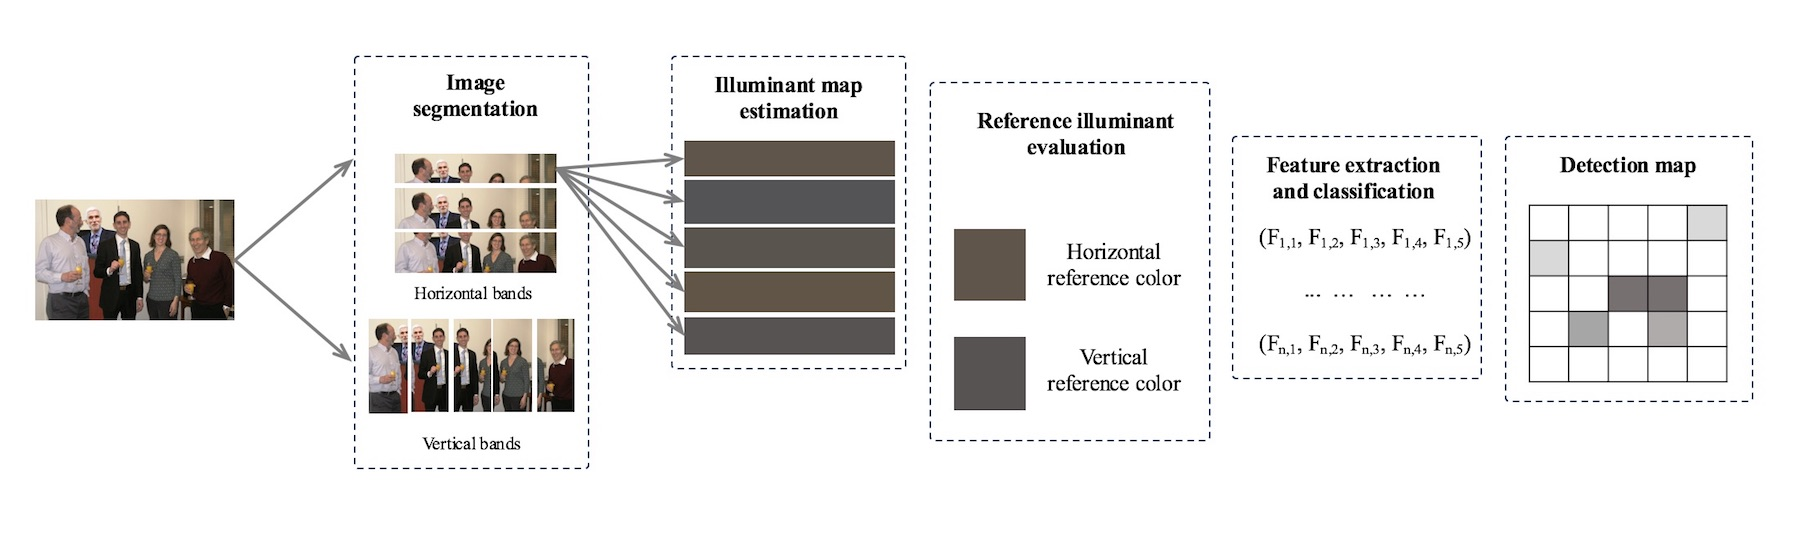
\includegraphics[width=1\textwidth]{images/pipeline_regions.jpg}
\end{center}
\end{tframe}

\begin{tframe}{Experimental results - 1}
\begin{table}[h!]
\centering
\begin{tabular}{l c c c c c} 
\hline \hline 
\textbf{Test case} & \textbf{Train} & \textbf{Test} & \textbf{Accuracy} & \textbf{AUC} &\textbf{ F-Score} \\ [0.5ex]
\hline
Test 1 & DSO-1 & DSO-1 &	0.84 & 0.90	& 0.78\\
Test 2 & DSI-1 & DSI-1 &	0.89 & 0.92 & 0.89\\
Test 3 &	DSO-1 &	DSI-1 &	0.59 & 0.58 & 0.64\\
Test 4 &	DSI-1 & DSO-1 & 0.63 & 0.60 & 0.54\\ [1ex]
\hline
\end{tabular}
\caption{Performance of face forgery detection module over paired faces using non-uniform weights.}
\end{table}
\end{tframe}


\begin{tframe}{Experimental results - 1}
\begin{table}[h!]
\centering
\begin{tabular}{l c c c c c} 
\hline \hline 
\textbf{Test case} & \textbf{Train} & \textbf{RC} & \textbf{ACC} & \textbf{AUC} &\textbf{ F-Score} \\ [0.5ex]
\hline
Test 1 & - & Median & 0.49 & 0.32 & 0.25\\
Test 2 & - & Global & 0.52 & 0.40 & 0.27\\
Test 3 & SplicedCC & Median & 0.54 & 0.53 & 0.26\\
Test 4 & SplicedCC & Global & 0.57 & 0.57 & 0.31\\
Test 5 &	 SplicedDSO & Median & 0.53 & 0.50 & 0.27\\
Test 6 &	 SplicedDSO & Global & 0.61 & 0.63 & 0.33\\ [1ex]
\hline
\end{tabular}
\caption{Performance of region forgery detection module.}
\label{table:performanceregionaldet}
\end{table}
\end{tframe}

\begin{tframe}{Conclusions}
\begin{itemize}
\vspace{0.1cm}
\item Two different approaches for forgery detection are presented: a face forgery detection module and a generic region forgery detection module.
\vspace{0.1cm}
\item \emph{Illuminant maps} are used to entail the interaction between the light source and the objects contained in a scene.
\vspace{0.1cm}
\item Face module achieved most promising results, but it needs some \emph{a priori} knowledge about the content of the image.
\vspace{0.1cm}
\item \textbf{Future developments}: given that our method compares skin material, it is feasible to use additional body parts, such as arms and legs, to increase the detection and confidence of the method.
\vspace{0.1cm}
\item Further improvements can be achieved when more advanced illuminant color estimators become available.
\end{itemize}
\end{tframe}
